Nesse capítulo, apresentamos os fundamentos da Análise de Redes Sociais. A análise de redes sociais (ARS) é uma abordagem que tem suas raízes na Sociometria e na Teoria dos Grafos, que são de viés matemático, para analisar relações sociais (Recuero, Bastos e Zago, 2015). A ideia central é que os indivíduos, ou atores sociais, estão inseridos em estruturas complexas de relações com outros atores, e essas estruturas têm um papel fundamental no comportamento e na visão de mundo desses indivíduos.

\section{Teoria dos Grafos}
A Teoria dos Grafos é um framework matemático que estuda as relações entre objetos e as conexões entre eles. As origens desta teoria estão no trabalho de Euler e na solução que ele propôs para o enigma das Pontes de Königsberg. A história relata que a cidade de Königsberg seria atravessada por sete pontes e que popularmente havia um desafio de desenhar um caminho por ela onde cada uma das pontes seria atravessada uma única vez. Euler teria demonstrado que tal desafio era impossível de ser resolvido utilizando um grafo, dando assim origem à teoria.

No livro "Introdução à análise de redes sociais online" de Raquel Recuero, a autora discute a importância da ARS e da Teoria dos Grafos para a compreensão das redes sociais online. Ela explica que a ARS permite a análise sistemática de grupos sociais a partir de sua estrutura, através de medidas específicas. A autora também destaca que a análise de redes sociais nasce de um ramo interdisciplinar de pesquisa, cujas bases podem ser encontradas nas mais variadas ciências, principalmente no início do século XX, particularmente, a partir da década de 1930.

Um conceito fundamental na Teoria dos Grafos é o de um "grafo", que é uma estrutura composta por "vértices" (ou "nós") e "arestas" que conectam esses vértices. Formalmente, um grafo $G$ é definido como um par ordenado $G := (V, E)$ compreendendo um conjunto $V$ de vértices ou nós juntamente com um conjunto $E$ de arestas ou arcos, que são pares de vértices (Bondy/Murty, 1976).

Os grafos podem ser categorizados como direcionados ou não direcionados. Em um grafo direcionado, as arestas têm uma direção associada, indicando uma relação unidirecional. Em contraste, em um grafo não direcionado, as arestas não têm direção, sugerindo uma relação bidirecional (West, 2001). Em termos de redes sociais, um exemplo de grafo direcionado seria o Twitter (onde um usuário pode seguir outro sem ser seguido de volta), enquanto um exemplo de grafo não direcionado seria o Facebook (onde a amizade é sempre mútua).

Outro conceito importante é o "grau" de um vértice, que é o número de arestas conectadas a ele. Em um grafo direcionado, distinguimos entre o "grau de entrada" (o número de arestas que entram no vértice) e o "grau de saída" (o número de arestas que saem do vértice). O grau de um vértice pode ser usado para medir sua importância ou influência dentro da rede (Newman, 2010).

Um "caminho" em um grafo é uma sequência de vértices na qual cada vértice é conectado ao próximo por uma aresta. O "comprimento" de um caminho é o número de arestas que ele contém. Este conceito é crucial para entender como a informação ou influência pode se propagar através da rede (Easley/Kleinberg, 2010).

A "conectividade" de um grafo é uma medida de quão integrada ou unida é a rede. Um grafo é dito "conectado" se houver um caminho entre cada par de vértices (West, 2001).

Um "subgrafo" é um grafo formado a partir de um conjunto de vértices e arestas de um grafo maior. Os subgrafos podem ser usados para estudar partes específicas de uma rede (West, 2001).

Recuero também enfatiza a diferença entre redes sociais e sites de rede social. Enquanto uma rede social está relacionada à percepção de um grupo social determinado pela sua estrutura (a “rede”), que é geralmente oculta, pois só está manifesta nas interações, as ferramentas sociais na internet são capazes de publicizar e influenciar essas estruturas sociais. Assim, o Facebook, por si só, não apresenta redes sociais. É o modo de apropriação que as pessoas fazem dele que é capaz de desvelar redes que existem ou que estão baseadas em estruturas sociais construídas por essas pessoas.

Portanto, a Teoria dos Grafos e a Análise de Redes Sociais são ferramentas essenciais para a compreensão das complexas redes de interações sociais que se formam tanto no mundo offline quanto online. Elas permitem uma visão mais profunda e sistemática das relações sociais, contribuindo para uma melhor compreensão dos fenômenos sociais.

\subsection*{Grafos Sociais}

Um dos primeiros desenvolvimentos na análise de redes foi o trabalho do sociólogo Georg Simmel no início do século XX. Simmel aplicou os princípios da teoria dos grafos às relações sociais, argumentando que as estruturas sociais surgem a partir dos padrões de interação entre os indivíduos \cite[]{2021_Hollstein}. Desde então, a análise de redes tem sido aplicada em uma ampla gama de campos, incluindo ciência da computação, física, biologia e ciências sociais, entre outros.

Simmel foi pioneiro em determinar a interação social como o bloco de construção básico da sociologia, indo além de seus contemporâneos, como Spencer. Ele argumentou que para entender o comportamento social, devemos estudar os padrões de interação, oferecendo insights penetrantes sobre a dinâmica das relações sociais. Embora Simmel nunca tenha usado o termo "rede social", muitos analistas de rede o consideram um precursor importante da abordagem de rede social.

Além disso, a análise de redes tem sido usada para entender a estrutura e a dinâmica de "redes escuras", como redes de criminosos ou terroristas. A análise de redes também tem sido aplicada para entender a estrutura e a dinâmica das organizações e como a estrutura da rede pode afetar a eficácia e a eficiência organizacional.

No entanto, apesar do rápido crescimento da análise de redes nas últimas duas décadas, as críticas à abordagem também aumentaram. Alguns críticos argumentam que a análise de redes pode ser excessivamente determinística, ignorando a agência individual e a complexidade das relações sociais (Scott, 1991). Além disso, a análise de redes pode ser desafiadora devido à dificuldade de coletar dados completos e precisos sobre redes sociais.

A análise de redes sociais tem sido criticada por sua falta de consideração pelos aspectos qualitativos das redes sociais e por sua tendência a simplificar as complexidades das interações sociais (Haythornthwaite, 2013). Além disso, a análise de redes sociais é frequentemente criticada por sua falta de consideração pelos aspectos contextuais das redes sociais e por sua ênfase excessiva em padrões estruturais (What is Social Network Analysis, n.d.).

Essas críticas destacam a necessidade de abordagens mais holísticas e integradas para a análise de redes sociais, que levem em consideração tanto os aspectos quantitativos quanto qualitativos das redes sociais, bem como os contextos sociais e culturais em que essas redes estão inseridas.

\subsection*{Centralidade e Comunidades}

Um método comum usado na análise de redes é a análise de centralidade, que mede a importância dos nós na rede com base em sua posição e conexões dentro da rede \cite[]{1978_Freeman}. Medidas de centralidade podem ajudar a identificar atores-chave na rede, ou nós que desempenham papéis importantes como porteiros, conectores ou intermediários entre diferentes partes da rede.

Outro método importante na análise de redes é a detecção de comunidades, que identifica grupos de nós que estão mais densamente conectados entre si do que com o restante da rede \cite[]{2004_Newman}. A detecção de comunidades pode ajudar a identificar grupos de indivíduos com atributos ou comportamentos semelhantes, ou grupos que são mais suscetíveis à propagação de informações ou influências.

\section{Aplicações da Análise de Redes}

A análise de redes tem sido aplicada em uma ampla gama de campos, além das redes sociais, com aplicações que vão desde redes de transporte até a neurociência. No campo do transporte, a análise de redes tem sido usada para estudar o fluxo de tráfego nas estradas e identificar áreas de gargalo que podem ser melhoradas para aumentar a eficiência do tráfego \cite[]{2012_Levinson}. Por exemplo, \citeonline{2010_Bierlaire} aplicaram a análise de redes para otimizar o sistema de transporte público, reduzindo o tempo de viagem e melhorando a eficiência do serviço. No campo acadêmico, a análise de redes tem sido aplicada para estudar as redes de coautoria na publicação acadêmica. \citeonline{2001_Newman} utilizou a análise de redes para estudar os padrões de colaboração entre autores e a emergência de comunidades de pesquisa. No campo organizacional, a análise de redes tem sido usada para compreender a estrutura de padrões de comunicação formais e informais em organizações. \citeonline{2004_Cross_BOOK} utilizaram a análise de redes para entender como os indivíduos influenciam os processos de tomada de decisão e a emergência de estruturas de poder dentro das organizações. Na biologia, a análise de redes tem sido usada para estudar redes de interação de proteínas, redes regulatórias de genes e redes metabólicas \citeonline{2004_Barabasi} utilizaram a análise de redes para entender como as proteínas interagem entre si em uma célula, fornecendo insights sobre como as doenças afetam essas interações.
\begin{figure}[!htb]
    \caption{Imagem ilustrativa de uma rede de interação de proteínas}
    \label{fig:network_proteins}
    \centering
    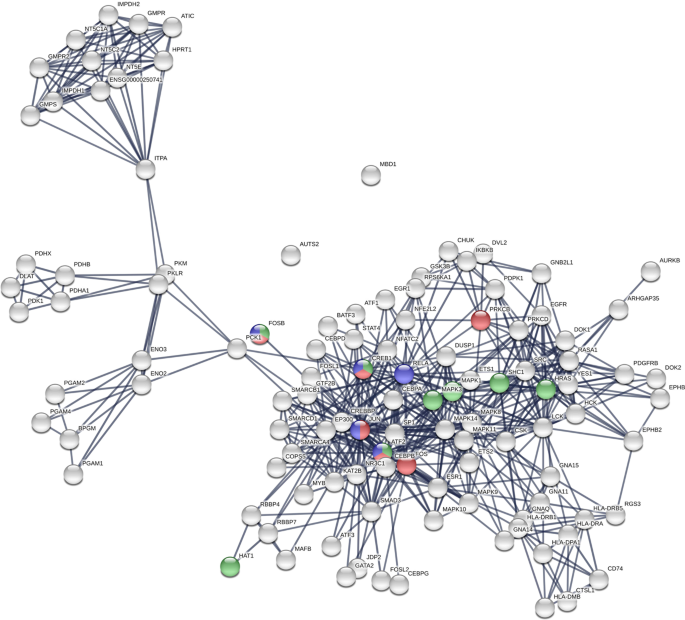
\includegraphics[scale=0.5]{network_proteins.png}
    \fdireta{2004_Barabasi}
\end{figure}
A análise de redes também tem sido usada em neurociência para estudar redes cerebrais. Por exemplo, pesquisadores têm utilizado a análise de redes para entender como diferentes regiões do cérebro interagem entre si, o que pode ajudar a entender doenças como a esquizofrenia e o Alzheimer \cite[]{2009_Bullmore}.
\begin{figure}[!htb]
    \caption{Imagem ilustrativa de uma rede de interação de proteínas}
    \label{fig:network_brain}
    \centering
    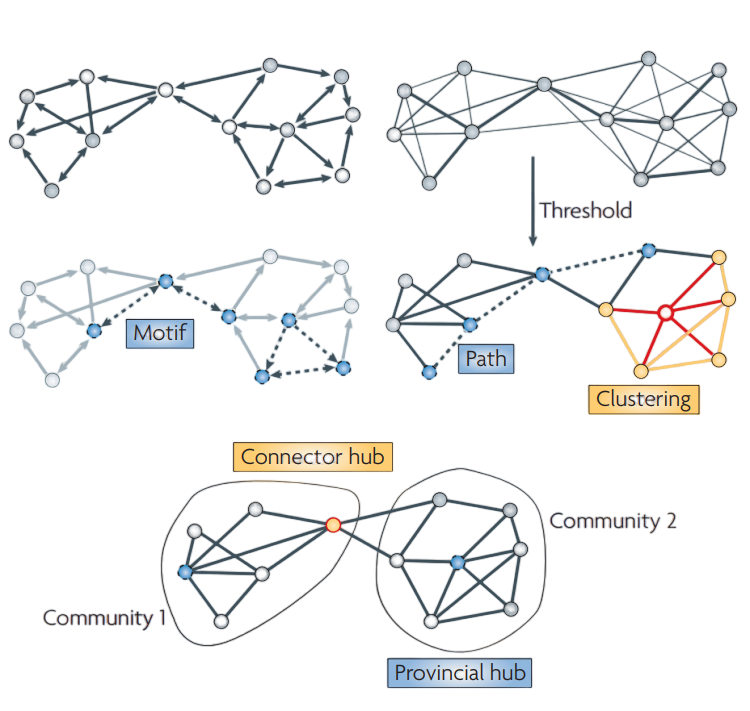
\includegraphics[scale=0.25]{network_brain.png}
    \fdireta{2009_Bullmore}
\end{figure}

\subsection*{Epidemiologia e Redes Complexas}
Na epidemiologia, a análise de redes tem se mostrado uma abordagem fundamental para estudar a transmissão de doenças infecciosas e entender a estrutura dos contatos entre indivíduos infectados. Dentre as diversas contribuições nesse campo, destaca-se o livro "Mathematics of Epidemics on Networks" \cite[]{2017_Kiss_BOOK}, que explora a aplicação do modelo SIR (Susceptível-Infectado-Recuperado) em redes complexas, em que os nós representam indivíduos e as arestas representam as interações entre eles. O livro desvenda como a estrutura da rede pode influenciar a propagação de doenças, investigando questões como o papel dos nós centrais na disseminação das enfermidades, a eficácia de diferentes estratégias de controle e intervenções, bem como o impacto de características topológicas específicas na dinâmica das epidemias. Uma das contribuições centrais do livro é a introdução do conceito de estrutura de redes em formato de gravata borboleta, a qual permite uma análise mais profunda e abrangente das redes complexas. 
Essa estrutura é composta por três principais componentes: a Área Central (SCC), a Seção de Entrada (IN) e a Seção de Saída (OUT). Matematicamente, podemos representar esses componentes de acordo com o seguinte modelo:

\begin{equation}
\text{{SCC}} = { v \in V : \forall u,w \in \text{{SCC}}, \text{{existe um caminho direto de }} u \text{{ para }} w }
\end{equation}

\begin{equation}
\text{{IN}} = { v \in V : \exists u \in \text{{SCC}}, \text{{ tal que }} (u,v) \in E \text{{ e não existe um caminho direto de }} v \text{{ para }} u }
\end{equation}

\begin{equation}
\text{{OUT}} = { v \in V : \exists u \in \text{{SCC}}, \text{{ tal que }} (v,u) \in E \text{{ e não existe um caminho direto de }} u \text{{ para }} v }
\end{equation}

Onde $V$\simbolo{V}{Representa um conjunto de nós em um grafo} representa o conjunto de nós e $E$\simbolo{E}{Representa um conjunto de arestas em um grafo} o conjunto de arestas da rede. A Área Central {SCC} consiste em nós altamente conectados, em que há um caminho direto de um nó para qualquer outro nó da área central. A Seção de Entrada {IN} é composta por nós que possuem conexões direcionadas para a área central, mas não têm caminhos de retorno diretos para os nós da Seção de Saída {OUT} ou da área central. Analogamente, a Seção de Saída {OUT} inclui nós que têm conexões direcionadas da área central, mas não possuem caminhos de retorno diretos para os nós da Seção de Entrada {IN} ou da área central.

Essa estrutura de redes em formato de gravata borboleta tem o potencial de ser aplicada para interpretar grafos direcionados em redes sociais. Ao analisar uma rede social, podemos identificar a Área Central {SCC} como os indivíduos ou grupos altamente conectados que desempenham um papel central na propagação de informações ou influência na rede. A Seção de Entrada {IN} representa os nós que interagem com a Área Central, mas não possuem conexões diretas entre si. Esses nós podem desempenhar um papel crucial ao receber informações da Área Central e disseminá-las para outros nós da rede. Da mesma forma, a Seção de Saída {OUT} inclui os nós que têm conexões direcionadas para a Área Central, mas não estão diretamente conectados uns aos outros. Esses nós podem ser responsáveis por disseminar informações ou influência da Área Central para outras partes da rede.

A propagação de fake news em redes sociais pode ser comparada à disseminação de doenças infecciosas, em que a informação falsa se espalha de maneira semelhante a um contágio. A estrutura de redes em formato de gravata borboleta, descrita no livro, pode ajudar a identificar os nós centrais e influentes que desempenham um papel importante na disseminação de informações falsas. Além disso, a análise da dinâmica da propagação de fake news pode se beneficiar das técnicas e modelos matemáticos discutidos no livro para compreender a rapidez e o alcance dessa disseminação.

Uma outra contribuição importante é na epidemiologia não Markoviana. Os modelos estocásticos de epidemias não markovianas (Stochastic non-Markovian epidemics) são uma extensão dos modelos clássicos de epidemias, que consideram a dependência temporal e complexa das interações entre os eventos em um processo epidêmico. Esses modelos reconhecem que a probabilidade de transição entre estados pode depender do histórico completo de estados anteriores, levando em conta fatores como a história de exposição, imunidade adquirida e comportamentos individuais. Matematicamente, podemos representar um modelo estocástico de epidemia não markoviana como:

\begin{equation}
P(S(t+\Delta t), I(t+\Delta t), R(t+\Delta t)|S(t), I(t), R(t), \mathcal{H}(t))
\end{equation}

onde $S(t)$, $I(t)$ e $R(t)$ representam o número de indivíduos suscetíveis, infectados e recuperados no tempo $t$, respectivamente, e $\mathcal{H}(t)$ denota o histórico completo dos eventos até o tempo $t$.

A aplicação dos modelos estocásticos de epidemias não markovianas na análise de redes sociais pode fornecer insights importantes para entender fenômenos como polarização e câmaras de eco. Ao considerar a dependência temporal nas interações sociais, esses modelos podem capturar como a exposição a determinadas opiniões ou informações no passado influencia a propensão de um indivíduo em adotar ou compartilhar essas opiniões no futuro. Essa dependência temporal pode ser representada por meio de uma função de probabilidade condicional:

\begin{equation}
P(I(t+\Delta t)|I(t), \mathcal{H}(t))
\end{equation}

Essa abordagem permite investigar como a formação e a propagação de polarização e câmaras de eco ocorrem ao longo do tempo em uma rede social. Por exemplo, pode-se analisar como a exposição a opiniões semelhantes influencia a adesão a um grupo específico e a formação de câmaras de eco, onde informações são amplificadas e reforçadas dentro de determinados grupos, resultando em uma maior polarização entre eles. Além disso, a aplicação desses modelos permite explorar o papel dos nós centrais na disseminação de polarização, bem como o impacto de intervenções e estratégias de controle na quebra das câmaras de eco e na redução da polarização.

Dessa forma, a utilização de modelos estocásticos de epidemias não markovianas na análise de redes sociais oferece uma abordagem poderosa para investigar e compreender os mecanismos subjacentes à formação de polarização e câmaras de eco. A inclusão da dependência temporal e das interações complexas entre os indivíduos permite uma representação mais realista dos processos sociais em redes complexas, proporcionando insights valiosos para o desenvolvimento de estratégias de mitigação e intervenções eficazes no combate à polarização e à formação de câmaras de eco em redes sociais.

A integração de eventos estocásticos, no contexto das redes sociais, pode ser relacionada aos momentos de grande tráfego ou atividade intensa nessas plataformas. Esses eventos podem ser caracterizados por um aumento significativo no número de interações, compartilhamentos, curtidas e comentários em determinados conteúdos. Matematicamente, podemos representar esses eventos estocásticos como:

\begin{equation}
P(S(t+\Delta t), I(t+\Delta t), R(t+\Delta t)|S(t), I(t), R(t), \mathcal{H}(t), \mathcal{T}(t))
\end{equation}

onde $\mathcal{T}(t)$ denota o histórico completo dos eventos de tráfego e atividade na rede social até o tempo $t$.

A introdução de hashtags como dados de entrada nessa análise pode ser feita considerando-as como fatores de disseminação de informações análogos ao contágio na epidemiologia clássica. A presença e popularidade de uma hashtag específica podem influenciar a propagação de informações relacionadas a um determinado tópico na rede social. Isso pode ser representado matematicamente pela função de probabilidade condicional:

\begin{equation}
P(I(t+\Delta t)|I(t), \mathcal{H}(t), \mathcal{T}(t), \mathcal{C}(t))
\end{equation}

onde $\mathcal{C}(t)$ representa o conjunto de hashtags relevantes e populares até o tempo $t$.

A inclusão das hashtags nessa análise permite uma compreensão mais abrangente e precisa da disseminação de informações nas redes sociais. Elas atuam como marcadores temáticos e podem desempenhar um papel importante na formação de comunidades online, na viralização de conteúdos específicos e na amplificação de certas mensagens. As hashtags funcionam como vetores de contágio, direcionando a atenção dos usuários para tópicos específicos e influenciando a propagação de informações relacionadas.

Ao incorporar as hashtags como fator de disseminação de informação na análise estocástica de redes sociais, é possível investigar como sua presença e popularidade influenciam a adesão dos usuários a determinados tópicos, a propagação de informações e a formação de comunidades temáticas. A análise da dependência temporal e da interação complexa entre as hashtags e o histórico de eventos na rede social pode fornecer insights valiosos sobre a dinâmica da disseminação de informações e ajudar a identificar padrões de comportamento e tendências emergentes.

Em resumo, a integração de eventos estocásticos no contexto das redes sociais, juntamente com a consideração das hashtags como fator de disseminação de informação análoga ao contágio na epidemiologia clássica, permite uma análise mais abrangente e precisa da propagação de informações e da formação de comunidades temáticas. Essa abordagem contribui para a compreensão dos processos sociais em redes complexas, fornecendo insights valiosos para a identificação de tendências, a criação de estratégias de engajamento e o desenvolvimento de intervenções eficazes na disseminação de informações em redes sociais.

\citeonline{2005_Christley} utilizaram a análise de redes para entender como a gripe se espalha em uma população, o que pode ajudar a desenvolver estratégias de prevenção mais eficazes.
\begin{figure}[!htb]
    \caption{Ilustração esquemática de uma topologia em formato de gravata borboleta}
    \label{fig:network_bowtie}
    \centering
    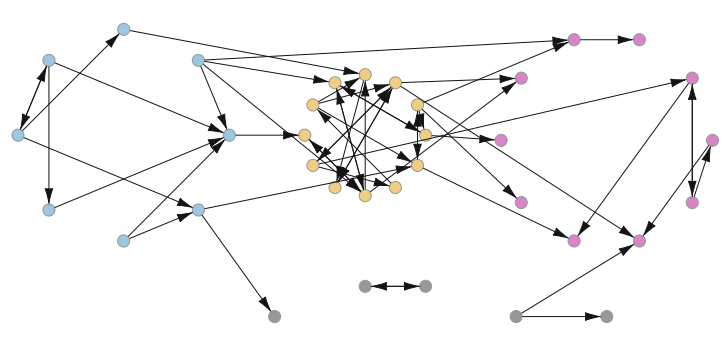
\includegraphics[width=\textwidth]{network_bowtie.png}
    \fdireta{2017_Kiss_BOOK}
\end{figure}

\subsection*{Análise de Redes Sociais Online}

Outra importante aplicação da análise de redes está no estudo de comunidades online e mídias sociais. O crescimento exponencial de plataformas online e redes sociais tem fornecido aos pesquisadores vastas quantidades de dados para analisar a dinâmica dessas comunidades. Por exemplo, um estudo de utilizou a análise de redes para investigar a estrutura e dinâmica das comunidades de discussão online no Reddit. O estudo constatou que as comunidades exibiam uma estrutura hierárquica com subcomunidades distintas que se formavam em torno de tópicos específicos. Outro estudo de \citeonline{2011_Quercia_IP} utilizou a análise de redes para estudar a influência de relacionamentos sociais na propagação de informações no Twitter. O estudo constatou que a estrutura da rede social influenciava a propagação de informações, sendo que clusters densamente conectados tinham maior probabilidade de promover a difusão de informações do que clusters esparsamente conectados.

Em conclusão, a análise de redes é uma ferramenta poderosa para analisar sistemas complexos e compreender as relações entre seus componentes. Ela tem suas origens na teoria dos grafos e se desenvolveu em um campo multidisciplinar com aplicações em várias áreas, como redes sociais, comunidades online, epidemiologia, ecologia e transporte. A aplicação da análise de redes em redes sociais tem levado a insights importantes sobre a estrutura e dinâmica dessas redes e tem ajudado os pesquisadores a compreender os mecanismos de influência social e a propagação de informações. O uso da análise de redes em outros campos também tem levado a descobertas importantes e tem o potencial de aprimorar nossa compreensão dos sistemas que moldam nosso mundo.

\subsection*{Análise de Redes Sociais no Brasil}

A \sigla{ARS}{Análise de Redes Sociais} emergiu como uma ferramenta poderosa e cada vez mais popular para analisar a estrutura e a dinâmica das redes sociais. Utilizada para estudar uma variedade de fenômenos, como comportamento organizacional, redes políticas, crime e inovação, a ARS tem demonstrado ser uma metodologia extremamente versátil. No Brasil, a relevância da ARS é evidenciada em múltiplos contextos e áreas de estudo, incluindo o planejamento urbano, a avaliação de políticas públicas, a compreensão das dinâmicas de migração e a análise de preconceitos e divisões sociais nas redes sociais [1, 2, 3, 4, 5].

Um dos aspectos que torna a {ARS} especialmente relevante no Brasil é o alto uso de redes sociais pela população. O Brasil é um dos países com maior número de usuários de redes sociais no mundo, criando um vasto campo de dados que pode ser analisado através da {ARS}. Além disso, a diversidade cultural e regional do Brasil, com suas muitas diferenças locais, proporciona um cenário complexo que a ARS pode ajudar a decifrar. Ao identificar padrões de interação e circulação de informações nas redes sociais, a ARS pode revelar como essas diferenças regionais e culturais se manifestam online.

Além disso, o Brasil enfrenta uma série de questões sociais complexas e uma alta polarização política, aspectos que são frequentemente expressos e amplificados nas redes sociais. A ARS pode ser uma ferramenta valiosa para entender a formação e a dinâmica dessas polarizações, assim como para estudar a formação de grupos de opinião e a disseminação de informações (ou desinformação). Por último, eventos de grande escala, como a Copa do Mundo, as Olimpíadas ou as eleições presidenciais, geram uma enorme quantidade de atividade nas redes sociais, proporcionando oportunidades únicas para a aplicação da ARS.

Diante deste cenário, este capítulo apresenta um resumo breve da de algumas contribuições relevantes que utilizam a ARS no Brasil, começando com uma revisão de suas principais contribuições teóricas e metodológicas. Em seguida, ele discute os desafios atuais e futuros na aplicação desta abordagem no contexto brasileiro, com o objetivo de explorar como a ARS pode continuar a fornecer insights valiosos em meio à constante evolução das redes sociais.

As contribuições teóricas e metodológicas da ARS no contexto brasileiro são diversas e significativas. A ARS tem sido aplicada em uma ampla gama de contextos, desde a análise de redes de colaboração científica até a exploração de redes de interação em plataformas de mídia social.

No campo teórico, a ARS tem contribuído para a compreensão de como as redes sociais influenciam uma variedade de fenômenos sociais. Por exemplo, o estudo de Melo et al. (2023) sobre a rede de interações no Twitter durante as eleições presidenciais de 2018 no Brasil contribuiu para a teoria da formação de grupos de opinião e da polarização política [6]. Da mesma forma, Santos et al. (2023) utilizaram a ARS para analisar a rede de interações no Facebook em uma comunidade quilombola no Brasil. Eles descobriram que a rede é altamente conectada, com uma forte presença de laços familiares e de amizade [7]. Este estudo ilustra como a ARS pode ser usada para entender a dinâmica das redes sociais em comunidades específicas, fornecendo insights valiosos sobre a estrutura e a dinâmica dessas redes.

Outro estudo relevante é o de Borges et al. (2023), que analisou a rede de interações no Twitter durante o \#ProtestodosPintas em Natal (RN) [11]. O estudo encontrou que os significados construídos nas redes sociais sobre o protesto foram em grande parte negativos, com a rede sendo articulada em torno dos perfis @tribunadonorte e @BlogdoBG. Este estudo demonstra como a ARS pode ser usada para analisar a opinião pública e a formação de consenso (ou dissensão) em torno de eventos específicos.

No campo metodológico, a ARS tem contribuído para o desenvolvimento de técnicas avançadas de análise de redes. Por exemplo, o estudo de Silva et al. (2023) sobre a rede de colaboração científica em pesquisas sobre a COVID-19 no Brasil utilizou técnicas avançadas de ARS para analisar a estrutura e a dinâmica da rede [8]. Da mesma forma, o estudo de Fonseca et al. (2023) sobre a disseminação de informações sobre a dengue no Twitter utilizou técnicas de ARS para analisar a propagação de informações e desinformação na rede [9].

A tese de doutorado de Renata Lopes Rosa (2016) também fez uma contribuição significativa para o campo metodológico, propondo novas métricas de sentimentos e afeto para melhorar a análise de sentimentos [10]. A métrica de análise de sentimentos associada a um fator de correção correspondente para n-gramas, tempos verbais, expressões e características pessoais, como idade, gênero e educação, é desenvolvida neste trabalho. As frases são classificadas em intensidade de sentimentos positivos, neutros ou negativos por meio de um novo dicionário de palavras em português e de um novo cálculo de sentimentos. A solução de análise de sentimentos e afeto é aplicada em um sistema de recomendação de músicas, como estudo de caso, que sugere conteúdos de acordo com o estado emocional da pessoa.

No entanto, a aplicação da ARS no contexto brasileiro também apresenta uma série de desafios. Primeiramente, a análise de redes sociais requer acesso a grandes volumes de dados, o que pode ser difícil de obter devido a questões de privacidade e ética. Isso é particularmente relevante no Brasil, onde a legislação de proteção de dados é rigorosa. A pesquisa de Oliveira et al. (2023) destaca esse desafio, discutindo a necessidade de desenvolver competências em ARS entre os profissionais de saúde para melhorar a gestão de sistemas de saúde [12].

Além disso, a análise de redes sociais pode ser complexa e requer habilidades técnicas e metodológicas avançadas. Isso pode ser um desafio no Brasil, onde a formação em métodos quantitativos avançados pode ser limitada. A pesquisa de Oliveira et al. (2023) destaca esse desafio, discutindo a necessidade de desenvolver competências em ARS entre os profissionais de saúde para melhorar a gestão de sistemas de saúde [12].

Outro desafio é a necessidade de adaptar a ARS para lidar com a constante evolução das redes sociais. Como Borges et al. (2023) apontam, as redes sociais estão em constante mudança, com novas plataformas emergindo e padrões de uso mudando ao longo do tempo. Isso requer que os pesquisadores estejam constantemente atualizando suas abordagens e técnicas de análise.

Finalmente, a diversidade cultural e regional do Brasil apresenta um desafio adicional. Como mencionado anteriormente, o Brasil é um país de grande diversidade, com muitas diferenças locais. Isso significa que a análise de redes sociais no Brasil deve levar em consideração essa diversidade, adaptando-se às especificidades de diferentes contextos regionais e culturais.

Apesar desses desafios, a ARS tem um grande potencial para contribuir para a compreensão de uma ampla gama de fenômenos sociais no Brasil. Por exemplo, a pesquisa de Gomes et al. (2023) sobre a rede de colaboração entre os pesquisadores brasileiros em Ciência da Informação demonstrou como a ARS pode ser usada para analisar a estrutura e a dinâmica das redes de colaboração científica [13].

Nesse contexto, uma pesquisa sobre a rede social Colab.re tem um potencial de se inserir de maneira relevante no cenário da Análise de Redes Sociais (ARS) no Brasil, um campo de estudo que tem visto aplicações diversificadas e significativas.

Assim como estudos anteriores, como o de Melo et al. (2023) e Fonseca et al. (2023), que exploraram a dinâmica das redes sociais durante eventos políticos importantes e a disseminação de informações e desinformação, o estudo busca entender a formação e a dinâmica das câmaras de eco. Este trabalho se alinha com os esforços anteriores para entender a polarização e a formação de grupos de opinião nas redes sociais.

Também aborda os desafios associados à aplicação da ARS no Brasil. Como Borges et al. (2023) apontam, as redes sociais estão em constante mudança, com novas plataformas emergindo e padrões de uso mudando ao longo do tempo. Ao focar em uma plataforma específica, a pesquisa do Colab.re responde a essa dinâmica, adicionando mais um pool de dados para o corpo de conhecimento da ARS no Brasil tanto de forma quantitativa, através da disponibilização dos dados, quanto de forma qualitativa, provendo um framework para futuras análises.

Com base nos dados extremamente localizados do Colab.re, nos quais os usuários interagem e criam eventos relacionados a problemas específicos em suas cidades, como buracos nas vias, calçadas irregulares, descarte irregular de lixo, vazamentos de água e iluminação pública, é possível obter insights valiosos tanto no âmbito social quanto político.

Em termos sociais, a análise das interações e dos padrões de engajamento dos usuários pode revelar informações sobre a coesão social e a formação de grupos de interesse em nível local. Por exemplo, ao examinar as postagens sobre problemas específicos, como buracos nas vias, é possível identificar redes de interação entre os usuários que compartilham preocupações semelhantes. Essas redes podem revelar comunidades de interesse e fornecer insights sobre a participação cívica local e a busca de soluções colaborativas para questões cotidianas.

Do ponto de vista político, a análise das interações políticas no Colab.re pode fornecer informações sobre a polarização e a formação de grupos de opinião em nível local. Por exemplo, ao examinar as postagens relacionadas a políticas públicas, é possível identificar padrões de interação entre usuários com diferentes posições políticas. Esses padrões podem ajudar a compreender a dinâmica da polarização política em nível local e como isso influencia a deliberação pública e a tomada de decisões políticas.

Em suma, a análise dos dados do Colab.re sob uma perspectiva da ARS permite adquirir insights valiosos em diversos aspectos sociais e políticos, desde a coesão social em nível local até a dinâmica da polarização política. Ao estabelecer essas conexões, é possível obter uma compreensão mais abrangente e contextualizada das redes sociais e de como elas impactam a vida cotidiana e a tomada de decisões nas comunidades.

\section{Compreendendo Câmaras de Eco e suas implicações}
\label{05_echochambers}
As mídias sociais revolucionaram a forma como as pessoas se comunicam e interagem umas com as outras. No entanto, o lado negativo dessa revolução é a crescente polarização e isolamento das pessoas em câmaras de eco. Uma câmara de eco pode ser definida como um sistema fechado em que as pessoas interagem apenas com aquelas que compartilham das mesmas crenças, valores e ideologias, enquanto ignoram ou suprimem ativamente pontos de vista opostos \cite[]{2015_Bakshy}. O termo "câmara de eco" tem origem no conceito de uma câmara de reverberação sonora, onde as ondas sonoras são refletidas entre as paredes, amplificando e distorcendo o som original.

Câmaras de eco podem ter sérias implicações para a sociedade, pois limitam a exposição a perspectivas diversas, levando ao reforço de crenças existentes e à exclusão de pontos de vista alternativos \cite[]{2001_Sunstein_BOOK}. Isso pode contribuir para a criação de uma divisão ideológica, que pode prejudicar o diálogo construtivo e o compromisso, resultando em uma sociedade polarizada e fragmentada. Além disso, câmaras de eco podem levar à disseminação de desinformação, propaganda e notícias falsas, uma vez que os indivíduos dentro desses sistemas fechados têm menos probabilidade de verificar a veracidade das informações que corroboram suas crenças existentes \cite[]{2016_Vicario}.

Compreender os mecanismos por trás da formação e manutenção das câmaras de eco é crucial para lidar com as consequências negativas associadas a esses fenômenos. A formação de câmaras de eco pode ser atribuída a diversos fatores, incluindo os algoritmos utilizados pelas plataformas de mídias sociais, os vieses cognitivos dos indivíduos e a influência de líderes de opinião \cite[]{2016_Flaxman}.

Em termos de fatores algorítmicos, as plataformas de mídias sociais utilizam algoritmos personalizados que visam fornecer aos usuários conteúdo alinhado com seus interesses, crenças e preferências. Isso significa que os indivíduos têm maior probabilidade de serem expostos a conteúdos que reforçam suas crenças e valores existentes, levando à formação de câmaras de eco \cite[]{2015_Bakshy}.

Vieses cognitivos, como viés de confirmação e exposição seletiva, também podem contribuir para a formação de câmaras de eco, pois os indivíduos tendem a buscar informações que confirmam suas crenças pré-existentes, enquanto ignoram ou rejeitam informações que as desafiam \cite[]{2006_Taber}. Além disso, líderes de opinião ou indivíduos com alta influência social podem desempenhar um papel na formação e manutenção das câmaras de eco, pois podem moldar as crenças e atitudes de seus seguidores \cite[]{2015_Bakshy}.

Câmaras de eco são um fenômeno preocupante nas mídias sociais, pois podem levar à polarização e fragmentação da sociedade, além da disseminação de desinformação e propaganda. Compreender os mecanismos por trás da formação e manutenção das câmaras de eco é crucial para mitigar suas consequências negativas.